\documentclass[oneside]{hcmut-report}

\usepackage{codespace}
\usepackage[dvipsnames]{xcolor}
\usepackage[most]{tcolorbox}
\usepackage{array,booktabs,tabularx,multirow}
\usepackage{enumitem}
\usepackage{caption,float}
\usepackage[export]{adjustbox}

\geometry{paper=a4paper,left=2cm,right=2cm,top=1cm,bottom=1cm,includeheadfoot,headheight=34.8pt,headsep=12pt,footskip=30pt,asymmetric}
\definecolor{myblue}{RGB}{33,102,172}
\newtcolorbox{importantbox}{colback=Green!8,colframe=ForestGreen!80!black,boxrule=0.8pt,arc=1mm,left=3mm,right=3mm,top=1mm,bottom=1mm}

\coursename{CO5085 -- Deep Learning and Its Applications in Computer Vision}
\reporttype{Exercises Report}
\title{CO5085 Exercises Report}
\advisor{Dr. Le Thanh Sach and Dr. Nguyen Quoc Minh}
\stuname{Dinh Hoang Duy Khanh \quad 2670306}
\reportplace{Ho Chi Minh City}
\reporttime{November 2026}
\setcounter{tocdepth}{2}

\newcommand{\reportleftheader}{%
  \bfseries
  \begin{tabular}{rl}
    \begin{picture}(25pt,15pt)
      \put(0,-8pt){
\includegraphics[width=20pt]{graphics/hcmut.png}}
    \end{picture}
    \begin{tabular}{l}
      \ttfamily Ho Chi Minh City University of Technology \\[-5pt]
      \ttfamily Faculty of Computer Science and Engineering \\
    \end{tabular}
  \end{tabular}%
}
\fancypagestyle{plain}{%
  \fancyhf{}%
  \fancyhead[L]{\reportleftheader}
  \fancyfoot[L]{\raisebox{3pt}{\ttfamily CO5085 Exercises -- Semester HK261}}
  \fancyfoot[R]{\raisebox{3pt}{\ttfamily Page \thepage/\pageref{LastPage}}}
  \renewcommand{\headrulewidth}{0.4pt}%
  \renewcommand{\footrulewidth}{0.4pt}%
}
\AtBeginDocument{\pagestyle{plain}}

\begin{document}
\begin{titlepage}
\begin{center}
VIETNAM NATIONAL UNIVERSITY -- HO CHI MINH CITY \\
HO CHI MINH CITY UNIVERSITY OF TECHNOLOGY \\
FACULTY OF COMPUTER SCIENCE AND ENGINEERING
\end{center}
\vspace{0.5cm}
\begin{figure}[h!]
\centering
\includegraphics[width=4.5cm]{graphics/hcmut.png}
\end{figure}
\vspace{0.4cm}
\begin{center}
\begin{tabular}{c}
\multicolumn{1}{c}{\textbf{\Large CO5085 EXERCISES REPORT}}\\
~~\\ \hline \\[-2pt]
\textbf{\large DEEP LEARNING AND ITS APPLICATIONS}\\
\textbf{\large IN COMPUTER VISION}\\[4pt]
\textbf{\large \textit{Group: Traiblazer}}\\[-2pt]
\hline
\end{tabular}
\end{center}
\vspace{0.9cm}
\begin{table}[h]\centering
\begin{tabular}{rll}
\textbf{Instructors:} & Dr. Le Thanh Sach & \\
& Dr. Nguyen Quoc Minh & \\[8pt]
\textbf{Student:} & Dinh Hoang Duy Khanh & 2670306 \\
\end{tabular}
\end{table}
\vfill
\begin{center}{\footnotesize \textit{Ho Chi Minh City, November 2026}}\end{center}
\end{titlepage}

\section*{Member List and Workload}
\addcontentsline{toc}{section}{Member List and Workload}
\begin{center}
\small
\begin{tabular}{|c|p{3.2cm}|c|p{4.9cm}|c|}\hline
\textbf{No.} & \textbf{Name} & \textbf{Student ID} & \textbf{Main responsibilities} & \textbf{Contribution} \\\hline
1 & Dinh Hoang Duy Khanh & 2670306 & Build and run E1--E3, create figures, verify results, prepare the GitHub page, and write this report. & 100\% \\\hline
\end{tabular}
\end{center}
\clearpage
\begingroup\footnotesize\tableofcontents\endgroup
\clearpage

\section*{Introduction}
\addcontentsline{toc}{section}{Introduction}
This report completes Exercises E1, E2, and E3 of CO5085 with one shared small dataset: Fashion-MNIST. Fashion-MNIST contains $28\times28$ grayscale clothing images in ten classes. It is allowed by the exercise sheet, visually more varied than handwritten digits, and small enough for a beginner to run on a personal computer.

The official 60,000 training images are shuffled with seed 42, then split into 48,000 training images and 12,000 validation images. The official 10,000 test images are kept for final evaluation. The same split is used in every exercise, so comparisons are fair. All models use Adam with learning rate 0.001, batch size 256, and cross-entropy loss. E1 and E3 use three epochs. E2 uses two epochs because it contains three attention experiments. These short runs compare designs clearly; they do not claim a fully optimized benchmark score.

\begin{importantbox}
\textbf{How to read the results.} Validation accuracy is used during training to compare choices. Test accuracy is reported after an experiment completes. A parameter count is the number of learned values in a model. A confusion matrix shows which classes are confused instead of only showing one average score.
\end{importantbox}

\subsection*{Reproducibility and AI-use declaration}
The project uses direct PyTorch code. Run \texttt{python -m E1.run\_e1}, \texttt{python -m E2.run\_e2}, and \texttt{python -m E3.run\_e3} from the repository root. The first run downloads Fashion-MNIST. Figures and JSON metrics are saved in \texttt{reports/}. AI assistance was used to help organize code and explain concepts. The student reviewed the code, ran the experiments, and is responsible for understanding and defending every model, result, and conclusion in this report.

\clearpage
\section{E1 -- Softmax, MLP, and CNN}
\subsection{Objective and model design}
E1 requires three classifiers and a custom training loop. The shared loop in \texttt{common.py} is explicit: for each batch it predicts scores, computes cross-entropy loss, calls \texttt{loss.backward()}, then calls \texttt{optimizer.step()}. This makes the learning process visible instead of hiding it inside a high-level trainer.

The Softmax classifier flattens an image into 784 pixel values and uses one linear layer with ten outputs. The MLP also flattens the image, then uses hidden layers of 128 and 64 values with ReLU activation. The CNN keeps the image grid. It applies convolution, ReLU, and max-pooling twice before a small fully connected head. Convolution helps the CNN learn local edges and clothing shapes from nearby pixels.

\begin{figure}[H]\centering
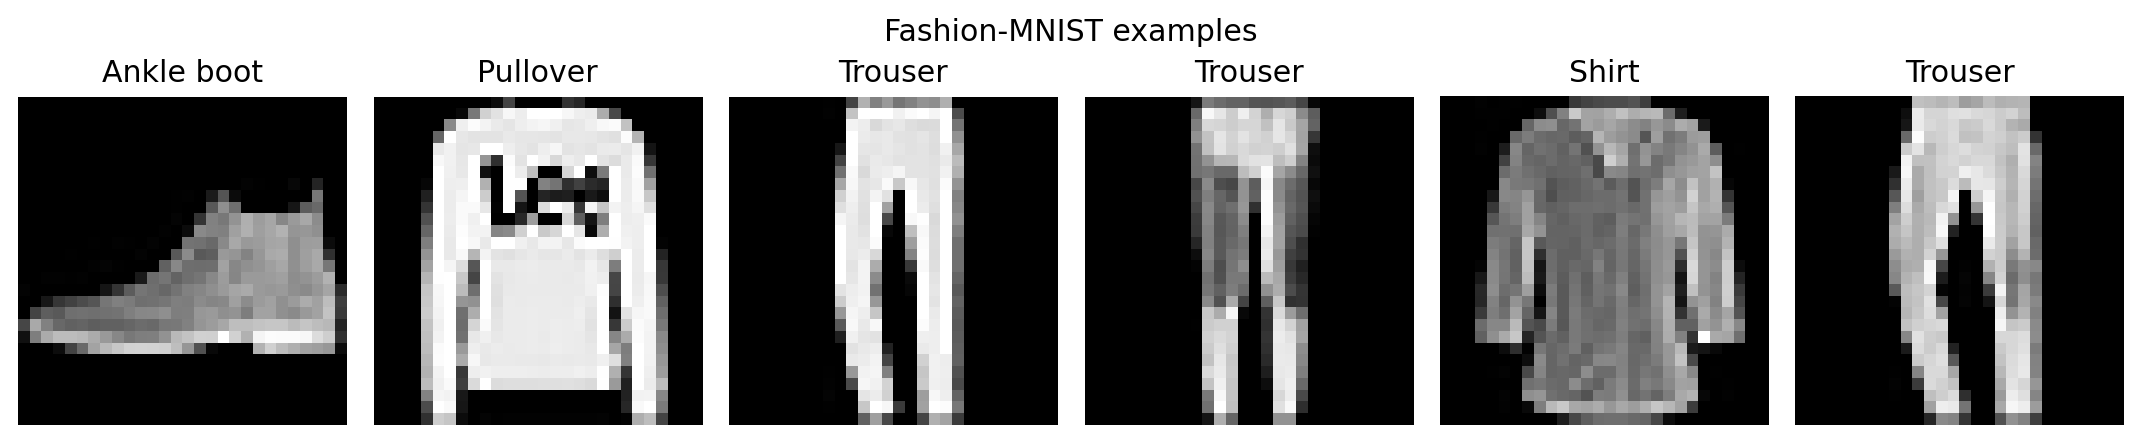
\includegraphics[width=0.74\textwidth]{images/e1_01_examples.png}
\caption{Examples from Fashion-MNIST. Each image has one clothing label.}\label{fig:e1-examples}
\end{figure}

\subsection{Results}
\begin{table}[H]\centering
\caption{E1 comparison on the same test set. Time includes training and evaluation.}\label{tab:e1-results}
\begin{tabular}{lrrr}\toprule
\textbf{Model} & \textbf{Parameters} & \textbf{Time (s)} & \textbf{Test accuracy} \\\midrule
Softmax linear & 7,850 & 125.2 & 0.8258 \\
MLP & 109,386 & 103.2 & 0.8518 \\
CNN & 105,866 & 156.4 & \textbf{0.8686} \\\bottomrule
\end{tabular}\end{table}

The CNN is best at 0.8686. It has nearly the same number of parameters as the MLP, so the improvement is not simply from a larger model. The CNN keeps local two-dimensional relationships; the MLP loses them when it flattens the image.

\begin{figure}[H]\centering
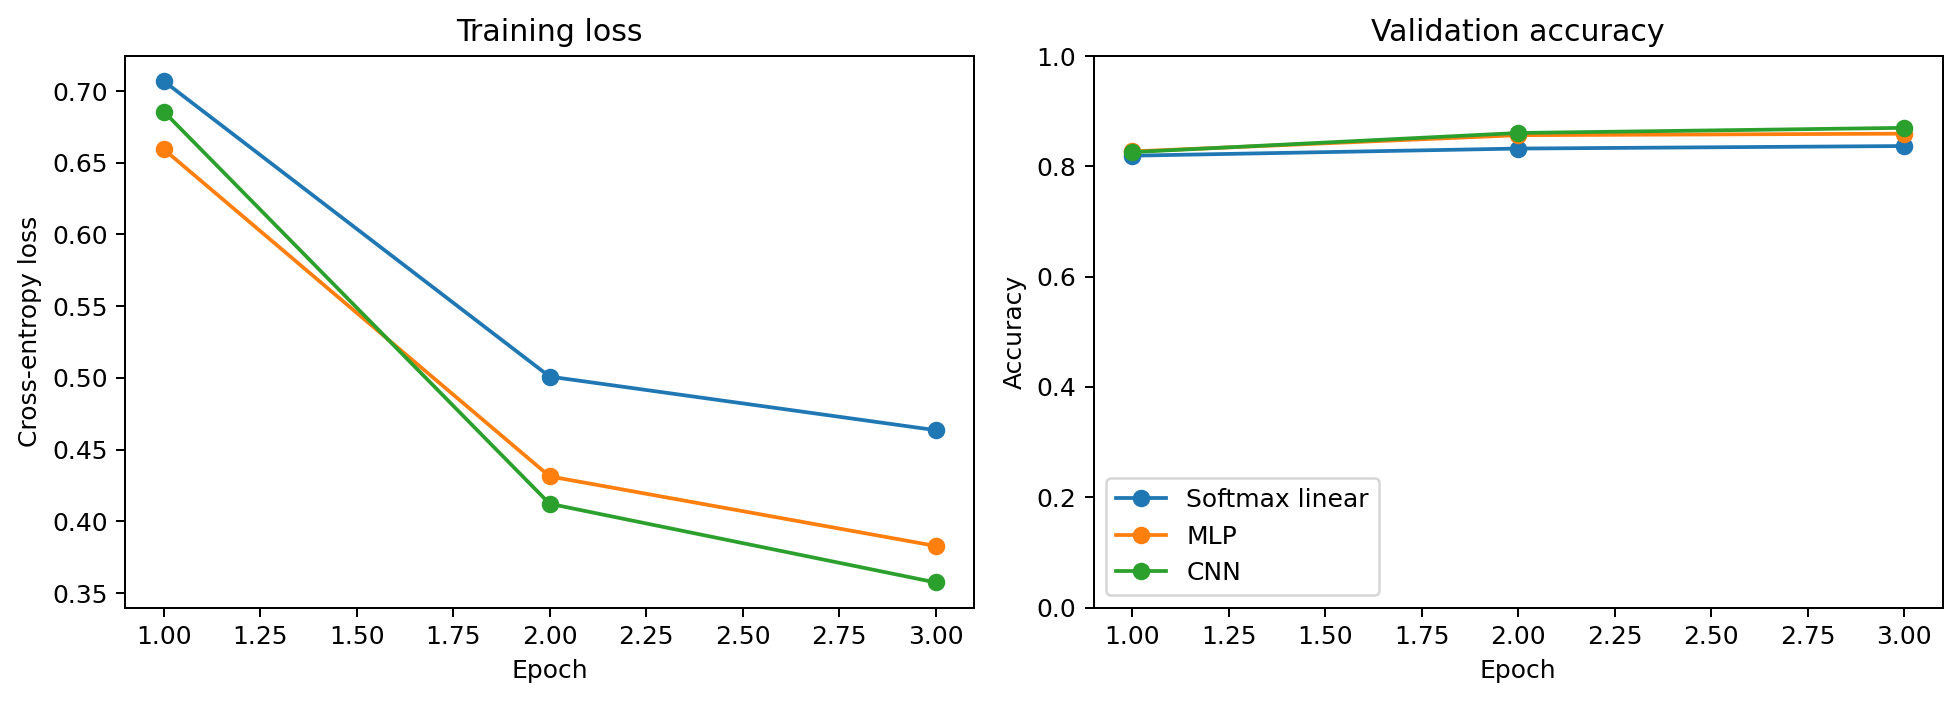
\includegraphics[width=0.88\textwidth]{images/e1_02_learning_curves.png}
\caption{Training loss and validation accuracy for E1.}\label{fig:e1-curves}
\end{figure}
\begin{figure}[H]\centering
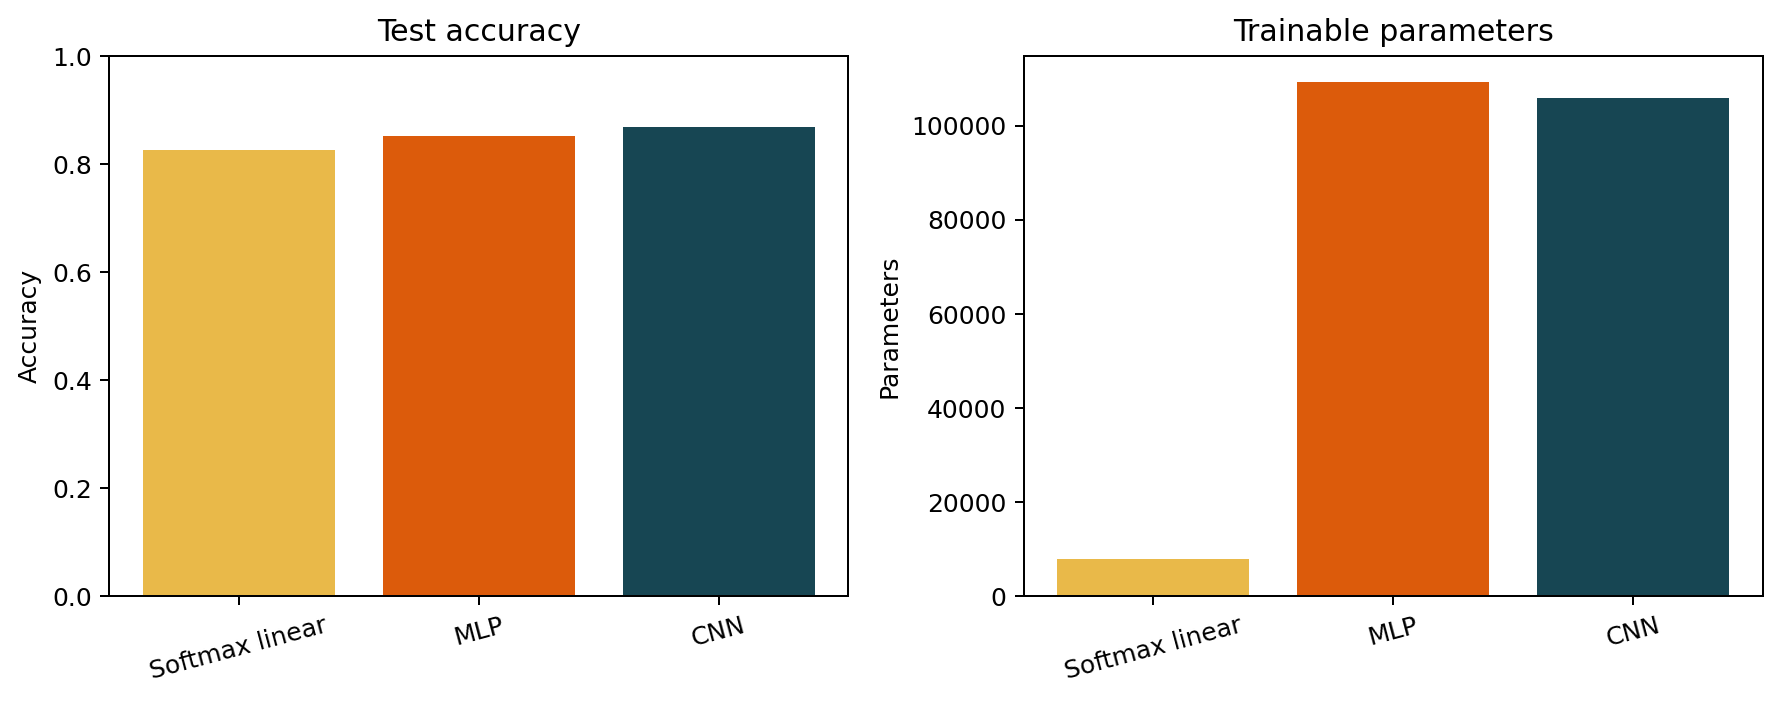
\includegraphics[width=0.74\textwidth]{images/e1_03_model_comparison.png}
\caption{E1 test accuracy and parameter comparison.}\label{fig:e1-comparison}
\end{figure}

\subsection{Error analysis}
The CNN confusion matrix in Figure~\ref{fig:e1-confusion} is calculated from the final test predictions. The diagonal contains correct predictions. Most off-diagonal errors are between visually similar upper-body classes such as shirt, T-shirt/top, pullover, and coat. This is reasonable because the images are grayscale and low resolution. Figure~\ref{fig:e1-errors} shows individual errors, which explains the score better than accuracy alone.

\begin{figure}[H]\centering
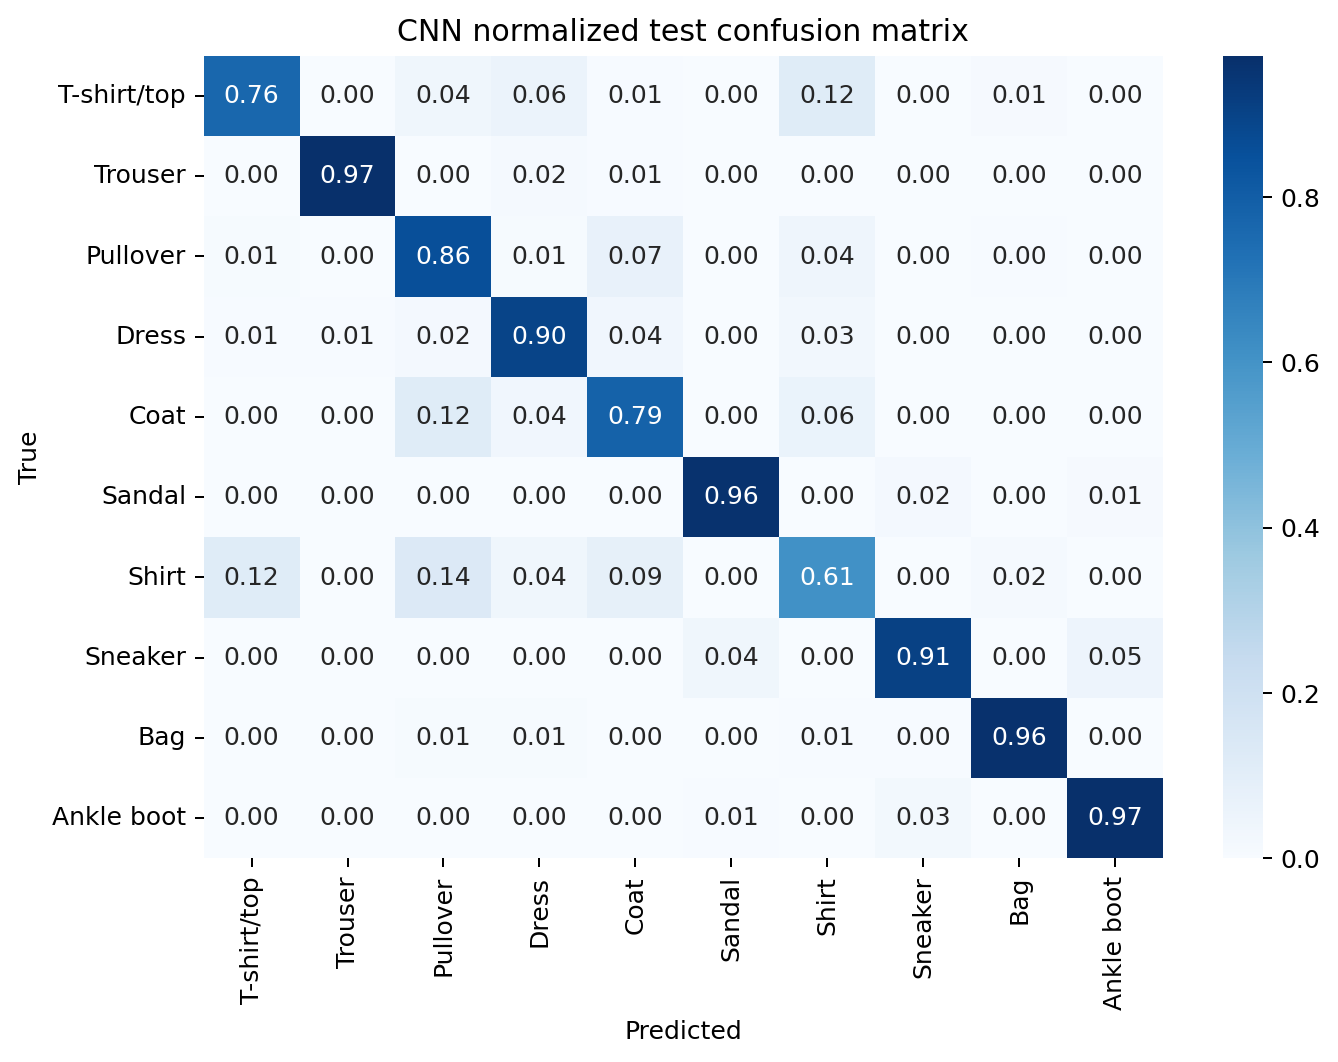
\includegraphics[width=0.70\textwidth]{images/e1_04_cnn_confusion_matrix.png}
\caption{Confusion matrix for the selected E1 CNN.}\label{fig:e1-confusion}
\end{figure}
\begin{figure}[H]\centering
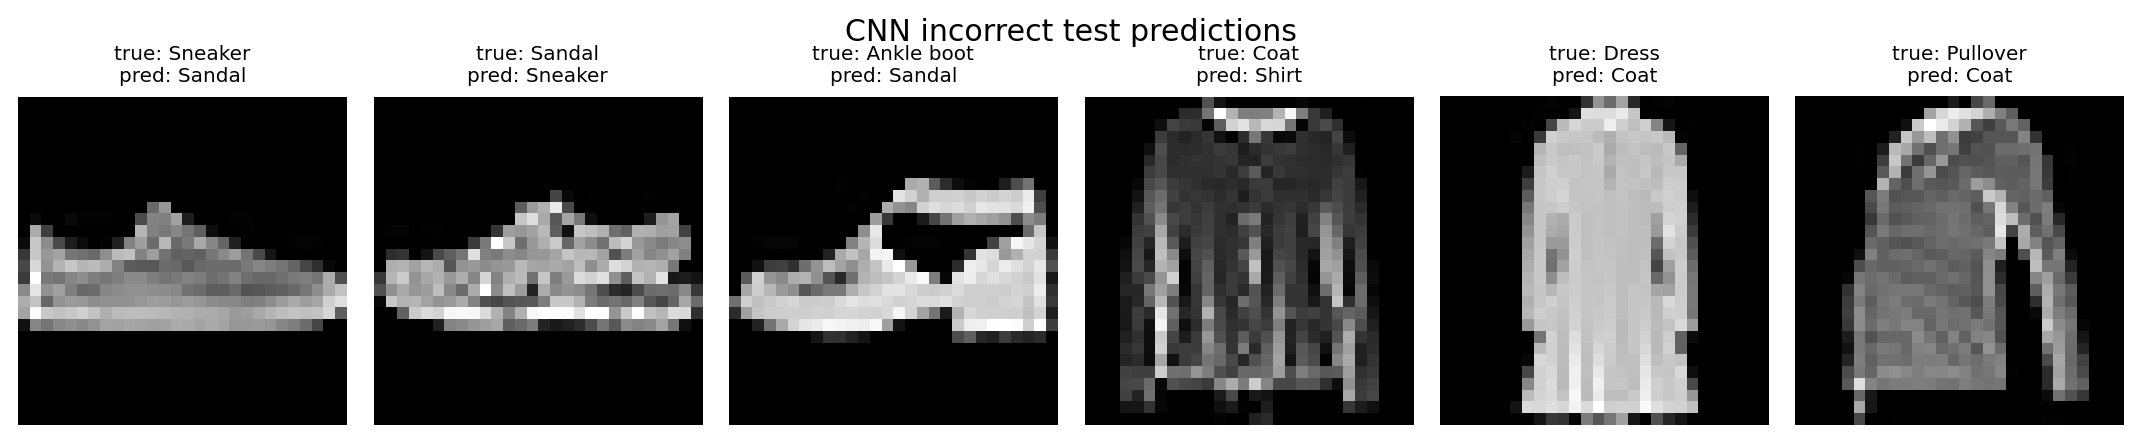
\includegraphics[width=0.88\textwidth]{images/e1_05_cnn_errors.png}
\caption{A small selection of CNN errors. Titles give true and predicted labels.}\label{fig:e1-errors}
\end{figure}

\clearpage
\section{E2 -- Multi-Head Self-Attention for Images}
\subsection{Tokens and attention}
Attention first needs a sequence of image tokens. The patch tokenizer cuts an image into 49 non-overlapping $4\times4$ patches and projects each patch to 32 values. The CNN-stem tokenizer uses two small convolution-and-pooling stages, then converts its $7\times7$ feature map into 49 tokens. The sequence length is the same, but the CNN stem supplies tokens that already contain local visual features.

\begin{figure}[H]\centering
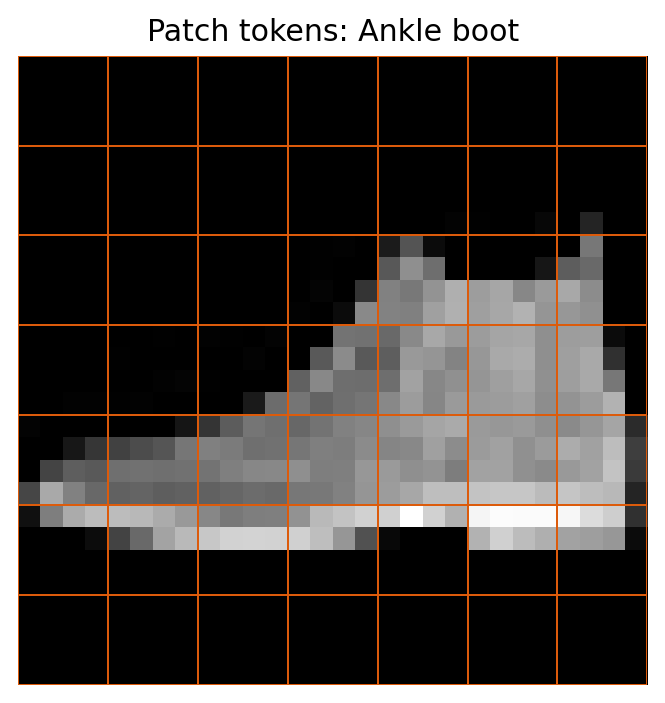
\includegraphics[width=0.52\textwidth]{images/e2_01_patch_tokens.png}
\caption{One image divided into 49 patch tokens.}\label{fig:e2-tokens}
\end{figure}

The manual MSA uses only linear layers, matrix multiplication, transpose, softmax, and reshape. For tokens $X$, it forms $Q=XW_Q$, $K=XW_K$, and $V=XW_V$. Attention weights are $\mathrm{softmax}(QK^T/\sqrt{d})$ and the output is a weighted sum of $V$. The code splits 32 values into two heads, computes each head, and joins them. It does not call \texttt{nn.MultiheadAttention}. The next experiment uses PyTorch MSA with the same patch tokens and settings. The third experiment changes only the tokenizer to the CNN stem.

\begin{table}[H]\centering
\caption{E2 attention and tokenization comparison; all runs use two epochs.}\label{tab:e2-results}
\begin{tabular}{lrrr}\toprule
\textbf{Model} & \textbf{Parameters} & \textbf{Time (s)} & \textbf{Test accuracy} \\\midrule
Manual MSA + patch & 10,986 & 110.7 & 0.7061 \\
PyTorch MSA + patch & 10,986 & 95.5 & 0.7072 \\
PyTorch MSA + CNN stem & 15,242 & 119.1 & \textbf{0.7578} \\\bottomrule
\end{tabular}\end{table}

Manual and PyTorch MSA with patch tokens have almost the same accuracy, 0.7061 and 0.7072. This is expected because their tokenization and architecture are matched. PyTorch MSA is a little faster. The CNN-stem tokenizer improves test accuracy to 0.7578 because it adds local edge and texture features before attention. The attention models remain below the E1 CNN because they are shallow and trained for only two epochs without augmentation or pretraining.

\begin{figure}[H]\centering
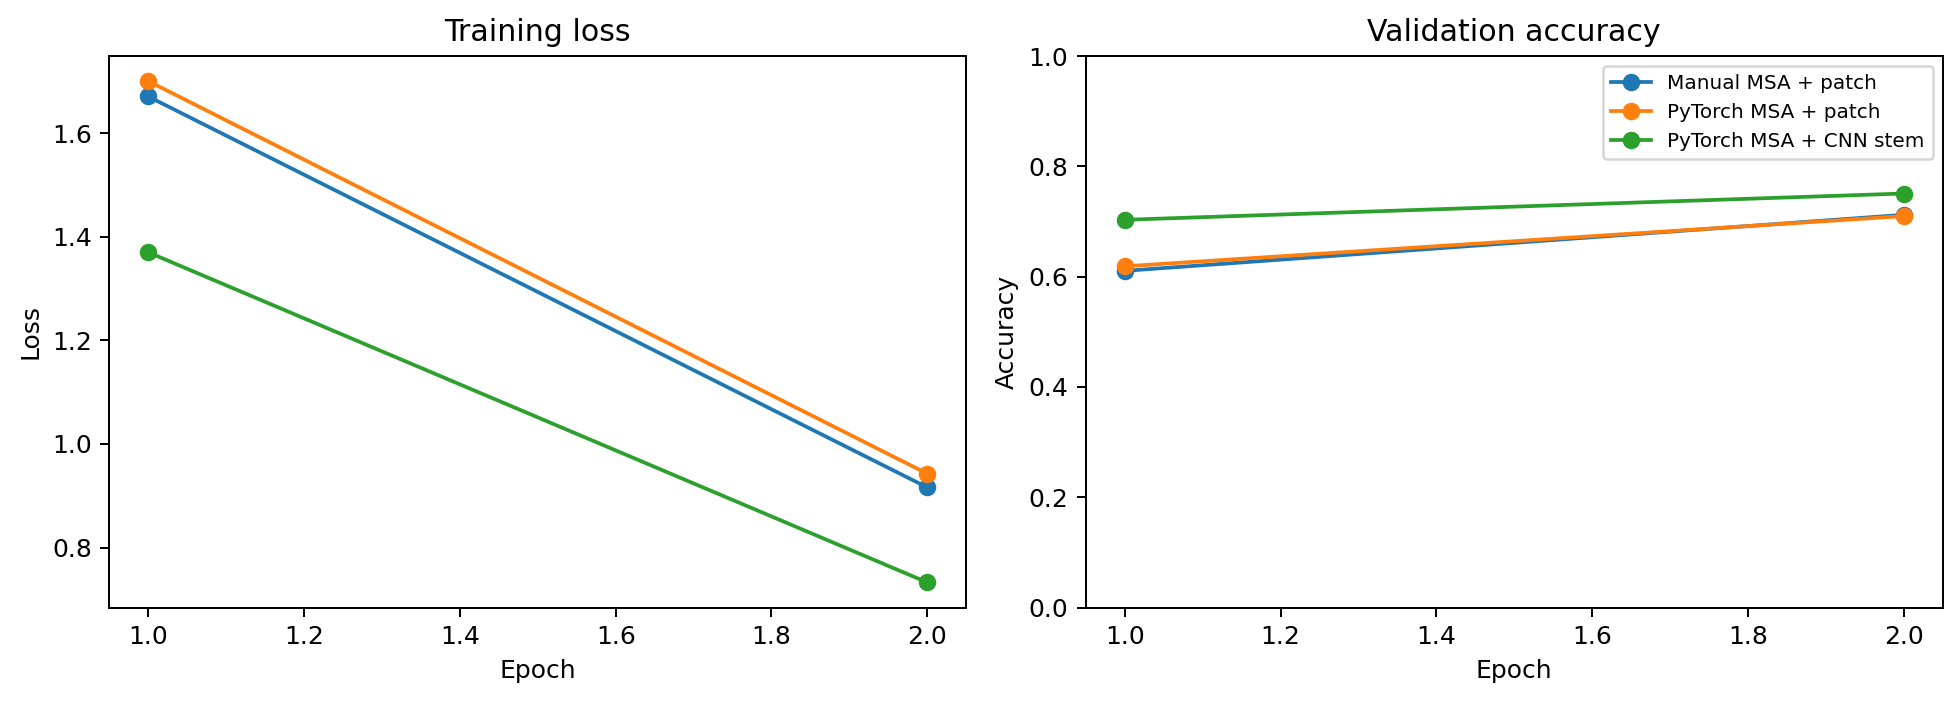
\includegraphics[width=0.86\textwidth]{images/e2_02_learning_curves.png}
\caption{E2 learning curves.}\label{fig:e2-curves}
\end{figure}
\begin{figure}[H]\centering
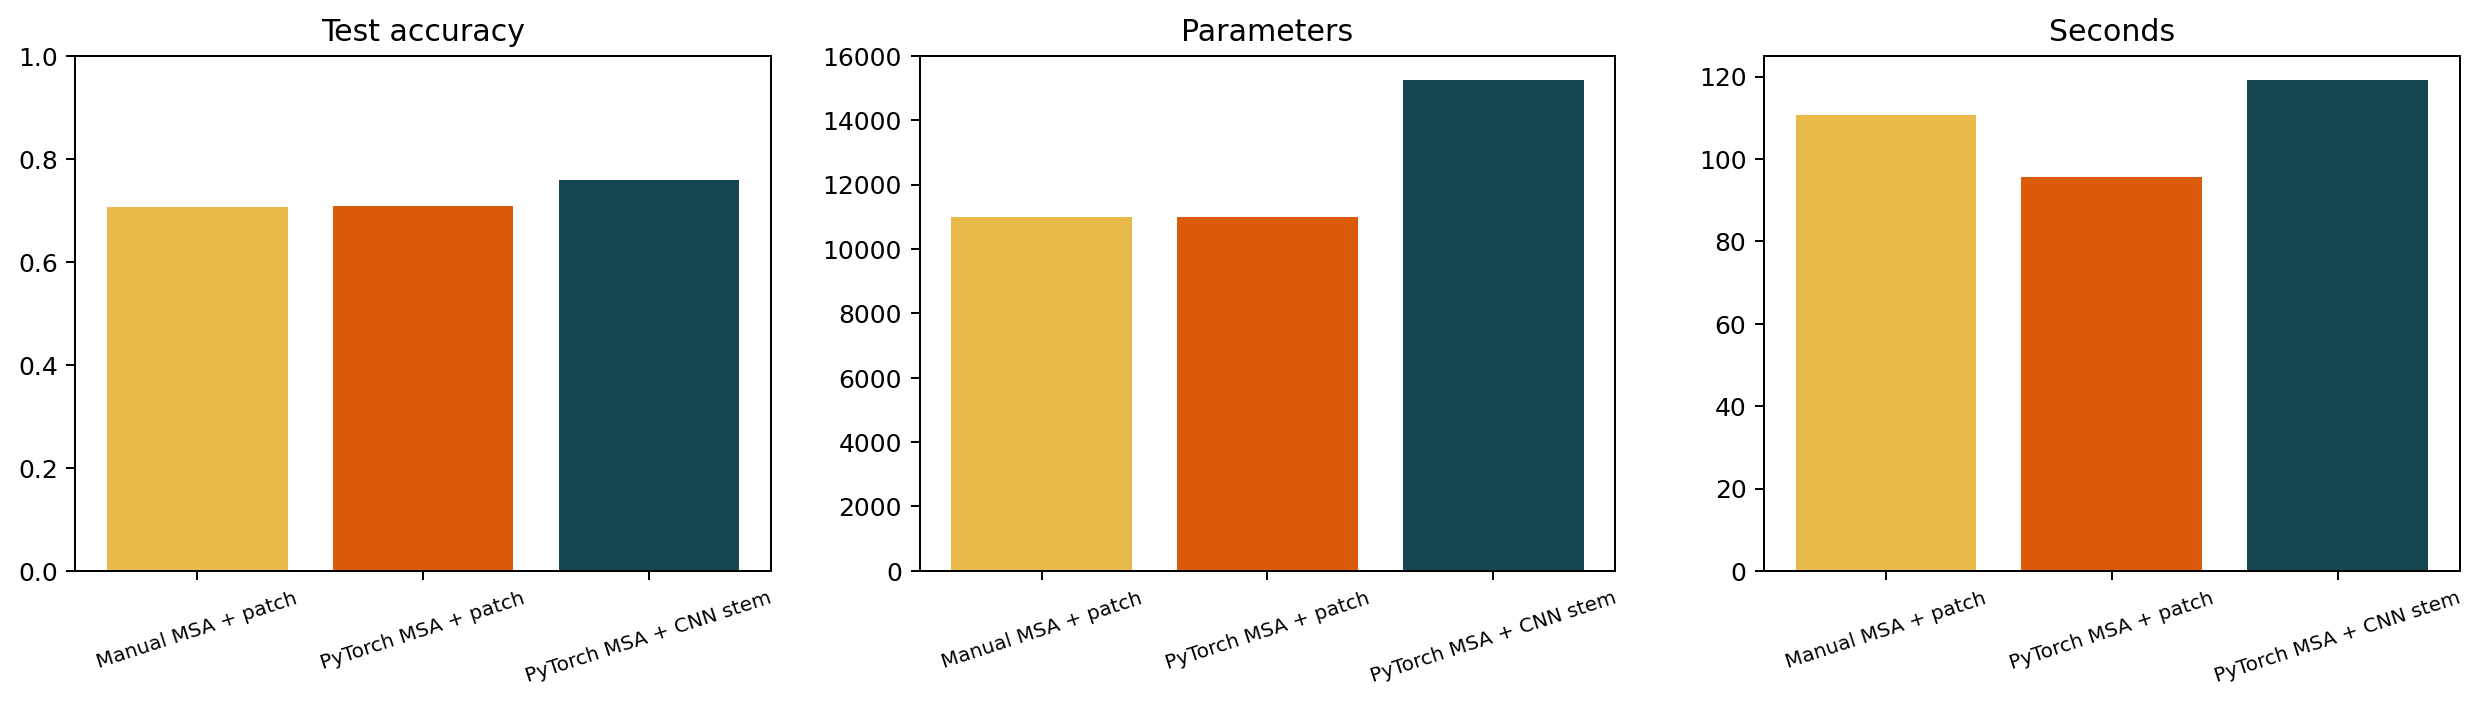
\includegraphics[width=0.76\textwidth]{images/e2_03_comparison.png}
\caption{E2 comparison of accuracy, parameters, and time.}\label{fig:e2-comparison}
\end{figure}
\begin{figure}[H]\centering
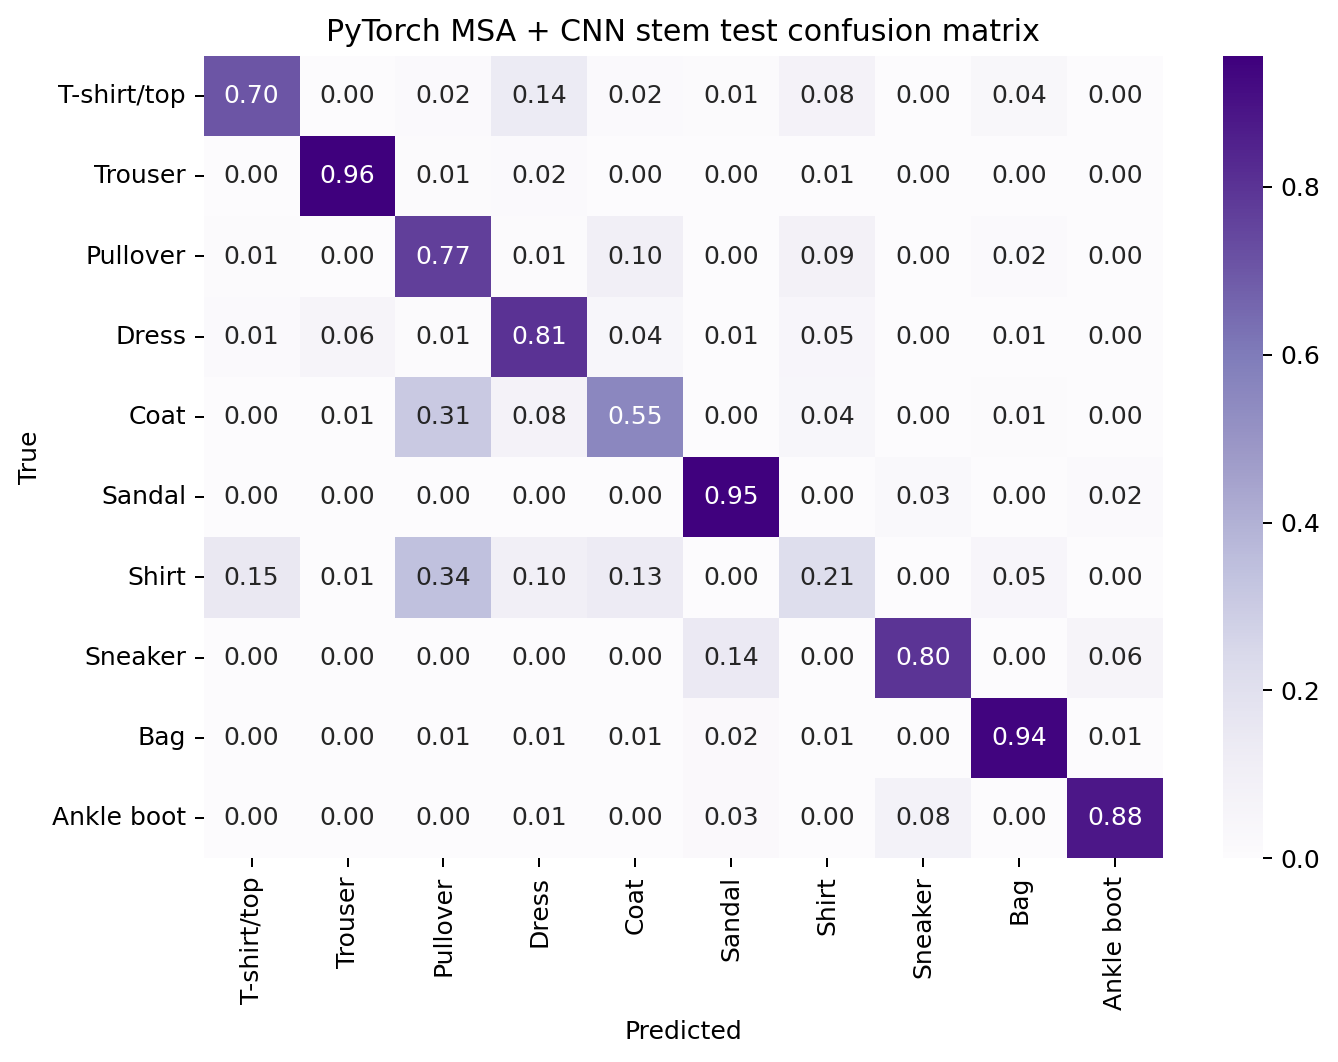
\includegraphics[width=0.70\textwidth]{images/e2_04_confusion_matrix.png}
\caption{Confusion matrix for PyTorch MSA with CNN-stem tokens.}\label{fig:e2-confusion}
\end{figure}

\clearpage
\section{E3 -- LSTM and GRU for Image Sequences}
\subsection{Image as a sequence}
E3 reads an image as a sequence instead of a grid. Each of the 28 image rows is one time step, and every step contains 28 normalized pixels. The sequence therefore has length 28 and input size 28. This is simple to implement, but it has a limitation: a recurrent model must compress earlier rows into a hidden state and does not naturally inspect nearby pixels in both directions as a CNN does.

\begin{figure}[H]\centering
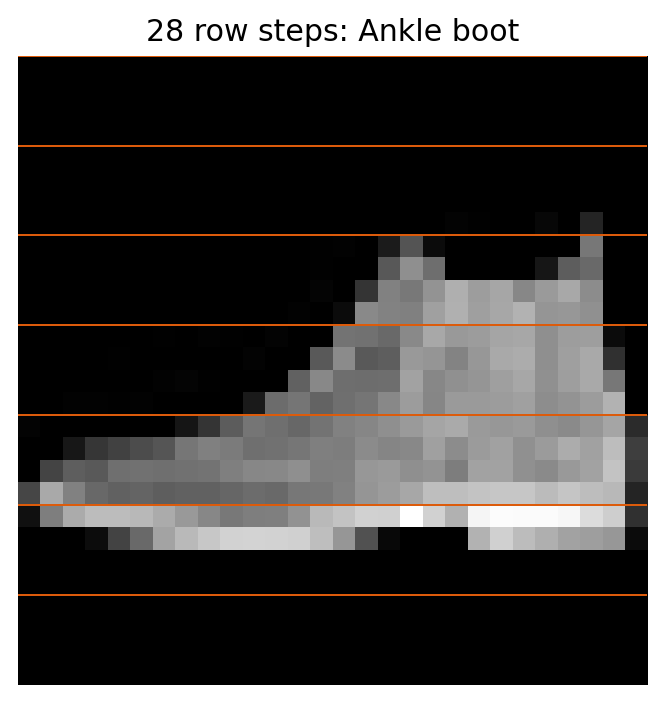
\includegraphics[width=0.46\textwidth]{images/e3_01_row_sequence.png}
\caption{Rows marked as time steps for LSTM and GRU.}\label{fig:e3-rows}
\end{figure}

LSTM and GRU both use hidden size 64 and a final linear classifier. The last recurrent output predicts the clothing class. LSTM has separate gates and a cell state, so it has more parameters. GRU combines some gates, so it is smaller. The E1 CNN result is the image-grid baseline.

\begin{table}[H]\centering
\caption{E3 recurrent models and the CNN baseline.}\label{tab:e3-results}
\begin{tabular}{lrrr}\toprule
\textbf{Model} & \textbf{Parameters} & \textbf{Time (s)} & \textbf{Test accuracy} \\\midrule
LSTM rows & 24,714 & 131.1 & 0.8201 \\
GRU rows & 18,698 & 102.6 & 0.8156 \\
CNN baseline (E1) & 105,866 & 156.4 & \textbf{0.8686} \\\bottomrule
\end{tabular}\end{table}

\begin{figure}[H]\centering
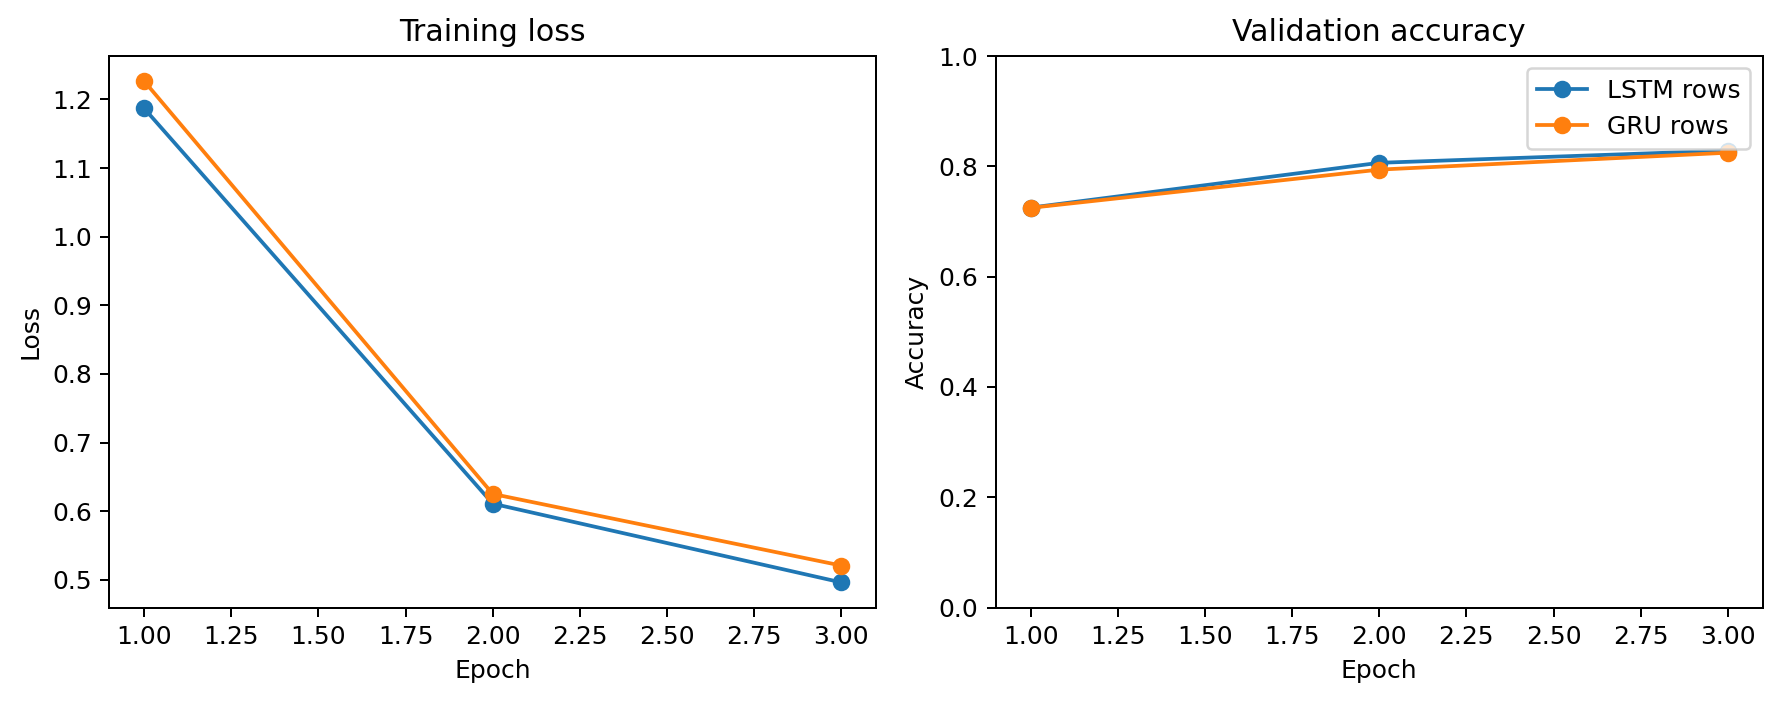
\includegraphics[width=0.86\textwidth]{images/e3_02_learning_curves.png}
\caption{LSTM and GRU training loss and validation accuracy.}\label{fig:e3-curves}
\end{figure}
\begin{figure}[H]\centering
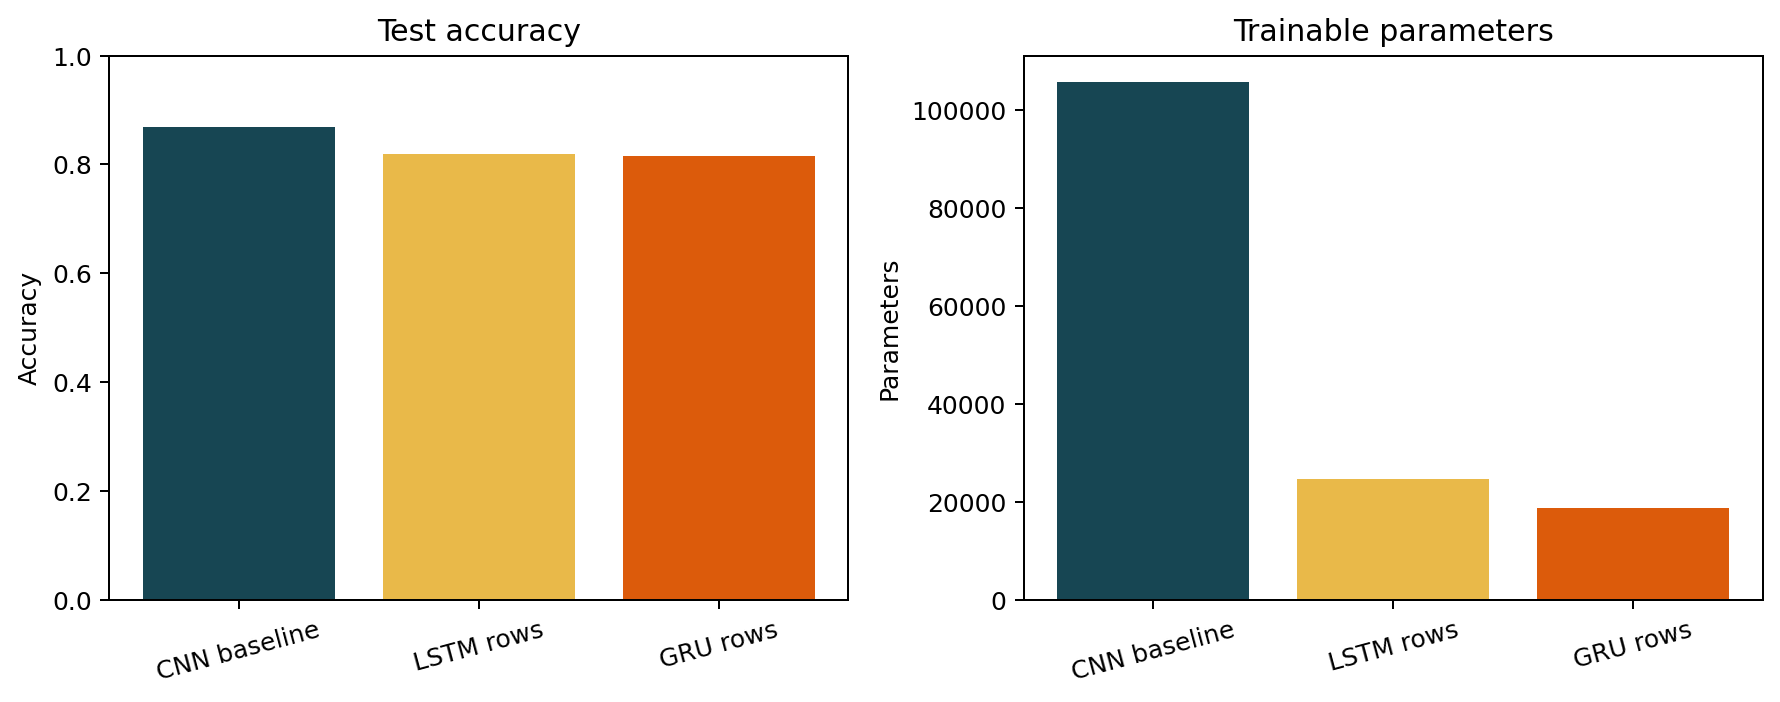
\includegraphics[width=0.74\textwidth]{images/e3_03_rnn_vs_cnn.png}
\caption{E3 accuracy, parameter, and time comparison.}\label{fig:e3-comparison}
\end{figure}

\subsection{Interpretation}
LSTM gives 0.8201 test accuracy and GRU gives 0.8156. GRU is faster and has fewer parameters, while LSTM is slightly more accurate. Both are below the CNN at 0.8686. The result supports the representation argument: CNN sees nearby pixels in height and width, while the row-sequence model has to remember earlier rows in a hidden state. RNNs are natural for sequence data; for these small images, CNN is the better choice.

\clearpage
\section{Requirement Checklist and Conclusion}
\begin{table}[H]\centering\small
\caption{Evidence that the exercise requirements are completed.}
\begin{tabularx}{\textwidth}{>{\bfseries}p{3.25cm}X}\toprule
\textbf{Requirement} & \textbf{Evidence} \\\midrule
One shared dataset & Fashion-MNIST and the same 48,000/12,000/10,000 split are used in E1--E3. \\
E1 models and errors & \texttt{E1/run\_e1.py}, Table~\ref{tab:e1-results}, curves, confusion matrix, and error samples. \\
Manual training loop & \texttt{common.py} explicitly runs forward, loss, backward, and optimizer step. \\
Manual and library MSA & \texttt{ManualMSA} uses matrix operations; the library comparison uses \texttt{nn.MultiheadAttention}. \\
Two tokenizations & Patch tokens and CNN-stem feature-map tokens; Table~\ref{tab:e2-results}. \\
LSTM, GRU, baseline & \texttt{E3/run\_e3.py} compares both recurrent units with the E1 CNN. \\
Reproducible delivery & Code, figures, JSON results, README, GitHub Pages source, and this PDF are stored together. \\\bottomrule
\end{tabularx}\end{table}

This project shows three ways to classify the same images. Softmax is the simplest baseline, the MLP learns nonlinear pixel combinations, and the CNN is strongest because it keeps the image layout. Manual attention agrees closely with PyTorch MSA, and CNN-stem tokens improve over raw patches. LSTM and GRU show how to read an image as a sequence, but CNN remains more suitable for this image dataset.

The code is intentionally short and direct. It shows the essential steps: prepare data, define a model, train with forward and backward propagation, evaluate a held-out test set, and inspect errors. Future work could add more epochs, augmentation, a deeper CNN, or a larger attention model. Those changes are outside this beginner-level submission.
\end{document}
